In this chapter we present our tactics and methods in regards to the collaboration. The level of abstraction is primarily on a descriptive level, while some challenges are also reflected upon. 

\section{Workflow} \label{sec:workflow}
For this project we decided to use an iterative design approach, both for the front-end and the back-end. Using this approach we were able to continuously evaluate both the concept and software.

We also used informal testing throughout the entire project. The goal here was to continuously test and optimize the software, learn about the stability and performance issues, so to finally adjust the implementation according to these findings.  An iterative design approach is commonly used for front-end design. It allows designers to identify usability issues that may arise in the user interface - before it is put into wide use. Even the best usability experts\footnote{We recognize Jakob Nielsen as a widely known usability expert.} cannot design perfect user interfaces in one single attempt. Hence a usability engineering life cycle should be built around the concept of iterations \cite{Nielsen1993}.

The figure below (fig. \ref{fig:workflow}) illustrates the different iterations, phases and stages of our project.

\begin{figure}[ht]
\centering
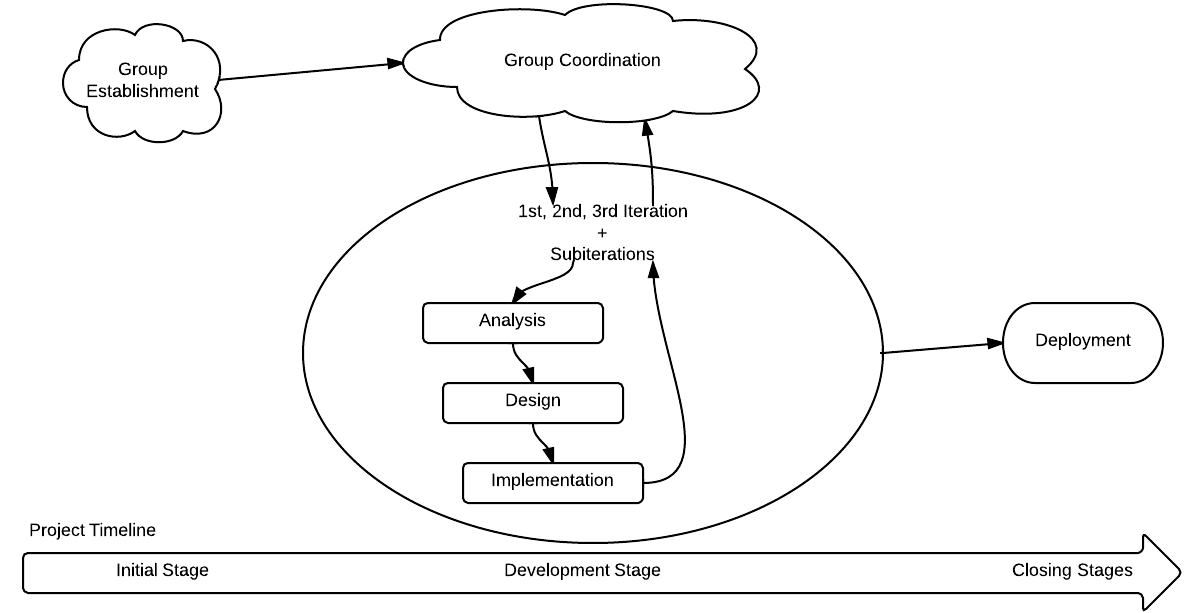
\includegraphics[width=\columnwidth]{images/workflow.png}
\caption{A generalized view of our workflow process}
\label{fig:workflow}
\end{figure}

Each of these illustrated elements were important for the process and contains all valuable information. Figure \ref{fig:workflow} contains a timeline, which chronologically shows, how the project evolved. The project went through three overall stages. These are known as the ``Initial Stage'', ``Development Stage'' and finally a ``Closing Stage''.

\subsection{Stages} \label{subsec:stages}

\subsubsection{Initial Stage}
Before the project kicked off and any kind of implementations began, we focused on how to handle the nine people in the group as \textit{one} collaborating team. 
This part was of high importance to us, being students with different nationalities, from far different continents. We didn't know anything about each other before hand. This made the task quite complicated. One could presume that in a normal work setting, at least the different roles in a team would already be settled. One could imagine that some people were hired to do the back-end (developer) and other people in charge of managing the project (project manager). 
We needed a specific initial stage to cover this part of getting to know each other, figuring out roles and knowledge areas of each team member. Within the group this was known as the ``Initial Stage''. The stage established the necessary basis to work as a team and made sure that project development went in the right direction to begin with.

\subsubsection{Development Stage}
During the development stage several iterations of analysis, design and implementation were executed. As figure \ref{fig:workflow} shows: The repetitive phases in the development stage is an iterative process. We went through this loop multiple times. To summarize we will describe three major iterations in the following section \ref{subsec:iterations}. 
The iterations are coherent with the project plan and present our general approach to the project. All of the three iterations contains multiple inclusive \textemdash by assessing the artefact\textemdash simpler iterations. Describing each iteration in detail would be a some what cumbersome process.

The reason for choosing three major iterations was to accommodate the overall deadlines for this project. Each deadline requested different material containing information about different levels of the project. The first deadline was focused on the requirements and motivation. The second delivery focused on related work and a project model, while the third delivery focused on the source code. These deadlines were a part of our overall project plan and thus led to having three overall deadlines. Initially our goal was to have four major iterations but this was changed due to our unsuccessful efforts to include our colleagues from Kenya. The postponement of deadlines and a general patient attitude caused us to eliminate one major iteration. 

The development stage contains furthermore a group coordination phase. The coordination is reached multiple times throughout the iterations. During this phase important topics were covered, such as sharing status, separation and distribution of tasks, figure out how to proceed, discuss upcoming challenges and the likes. Multiple collaboration methods and tools were used throughout this coordination phase (See \ref{sec:collaboration} and \ref{sec:tools}).

\subsubsection{Deployment Stage}
The deployment stage was considered the simplest and easiest to handle stage of our process. Upon reaching agreement that the development was finalized, the product was deployed to our server. This concluded our work on the product and finalized the development.

\subsection{Iterations} \label{subsec:iterations}
\subsubsection{First Iteration}
Our focus during the first iteration was to get the group work to flow and figure out how to handle the data services provided by the Danish university. Most of the iteration was related to get to know each other and figure out how to move the project forward. The artefacts produced here was of lower level, such as diagrams of the group members programming skills, use case diagrams, first thoughts of domain model, early prototypes of the frontend interface and early implementations of the data services.

It was difficult to really push the project forward at this phase. We used different means of communication with the Kenyans, but without any positive result. Our best result was reached when two out of four African members replied to our emails. No feedback, replies, comments or the likes was received from the two last members.

\subsubsection{Second Iteration}
During the second major phase the groups communication platform and general condition was stable - but unfortunately without any involvement from our Kenyan team members. We knew that we had to push the project forward, and had already wasted too much time on the effort to engage and activate unresponsive members. We were behind our project plan in an attempt to give them enough time to respond, without any luck. We tried to activate one semi-active member from Kenya as a team leader, but his response was, that he was not able to contact the other members.

Our focus changed from here. At the following team meeting we agreed upon, that it would be up to us, to get the project going. We chose to do so because of the fact that we did not receive any kind of feedback from Kenya. We would still let them know every step in the project, and we would continue to try to involve them as much as possible, by emailing them and the likes. We developed multiple artefacts at this point. Our goal through the second iteration was to get a working backend up and running. To do this, we had to chose the best fitting development platform and hereby programming language. The group had to agree on a set of requirements for the engine derived from the requirements in the assignment. The data model was completed and implemented, development of an early working prototype of the backend, and generated several jUnit tests to validate its robustness. Furthermore the work on the frontend started to take form. We did our first evaluation of the frontend (see \ref{sec:usability-test}).

\subsubsection{Third Iteration}
The third and final iteration was a hectic period with focus on getting things done and complete tasks. Because of the earlier effort to activate the Kenyan members, and the time consumed here, we were lacking behind. The now only moderate active member from Kenya chose to leave the group due to personal circumstances. The frontend was implemented with support from data provided by the backend. A second usability test was produced. Also this paper was mostly produced here, by combining bits and pieces and adding lots of new material. Finally the end product was deployed to our server.

During all of the iterations, both major and minor, we used a palette of different methods and tools. These are highly linked with the project phases. The most important are introduced and explained by usage, in the parts that follow below.

\section{Collaboration} \label{sec:collaboration}
A set of different methods were used during the initial stage, in the group establishment, and afterwards in the development stage. These were applied in order to promote and streamline collaboration. Several challenges were met and could have been solved by applying the correct mitigation strategy. The collaboration between the Danish and Kenyan team never evolved enough to engage some of the tactics. The following sections will only highlight the actual engaged methods, and will leave also leave out some methods that are only used briefly. This is done to inform which important actions were taken to engage the Kenyan members and not to blur the picture by which methods that could have been used at a later stage, if the collaboration evolved. 
%For a complete reference of all methods that we sought to use and how they could have been used, see Appendix \ref{sec:collaborationappendix}.

\subsection{Create a common platform} \label{sec:commonplatform}
At the time of the project start we were fully aware that we had several discontinuities, as described by Watson-Manheim et al. \cite{watson2007distance}, between the two groups. Too mention a few, the most challenging were, that we did not share the same culture, time zone \textemdash Kenya was ahead of two hours\textemdash, possibly skills, history and the likes. All of which makes it a challenge to collaborate. One way to solve this is to get to know the different team members in the group. The first step we took in order to make the group work as one unit was to try to create a common ground. The term to create common ground ``refers to that knowledge that the participants have in common, and they are aware that they have it in common'' \cite{olson:2000:distance}. The fact that the members in the teams, local as well as global, had not met each other, or collaborated, before, only stressed the importance of this. In a group like this, where members are spread across different continents, the common ground and the social context that ones behave in, is important. No one knew what to expect from each other, and different cultures introduces different challenges. 

Our approach to mitigate this problem was to email each member, by the email supplied by the coordinators, and introduce the members from ITU. The introduction was superficial and not exhaustive, in order not to frighten anybody. Basic information was listed, such as name, gender, age, contact methods and the likes. This would be a 30 seconds email to compose, and we nonetheless never received any replies. To mitigate this challenge of no replies, we tried to create a spreadsheet listing these simple informations, and expanded it with individual skills significant to the project. It took the Kenyan members close to two weeks to complete this form, while others never completed it.

The reasoning for collecting the members individual skills was to figure out which platform to develop on. In the beginning of the project we talked about the many technologies available for web development. There are many approaches to the same solution, with their pros and cons. Focusing on working as a team, with different members that all have considerably different background experiences we decided to individually write down our development qualifications.

The results were collected and top three choices were joined in a table (See Table \ref{tbl:dev_environment}). Every member then voted for the preferred development platform. One (1) being the preferred approach and three (3) the least preferred. The results are shown below:

\begin{table}[ht]
\caption{Members preferred development platform}\label{tbl:dev_environment}
	\begin{tabular}{rccccccccc}
	& \rotatebox{90}{Kasper} & \rotatebox{90}{Thomas} & \rotatebox{90}{Stefan} & \rotatebox{90}{Rasmus} & \rotatebox{90}{Nicolas} & \rotatebox{90}{Steven} & \rotatebox{90}{Cecil} & \rotatebox{90}{Tom} & \rotatebox{90}{Lucy} \\
		PHP 			& 2      & 1      & 3      & 3      & 1   		&1 			&3	 		&-	 		&1	\\
		C\#.Net   & 3      & 3      & 2      & 1      & 3    		&3 			&2 			&- 			&3  \\
		Java      & 1      & 2      & 1      & 2      & 2     	&2 			&1 			&- 			&2	\\
	\end{tabular}
\end{table}

\textit{Note: Tom in table \ref{tbl:dev_environment} did not share his experience with the team. Therefore the comparison table was never fully completed.}

The table shows a total score of of 20 points to C\#, 15 points to PHP and finally 13 points to Java, where lower is better. This indicates that Java could be the right choice for our group.

One of the challenges in this project was technology readiness \cite{olson:2000:distance}. Every team member has a preferred development language, which ultimately led to a long debate on settling with a development language, and what kind of framework the group should use. The problem was that some team members would have some difficulties participating in the development because of the fact that not all had the same preferred language.

Also some members already had some experience in development of web applications, while others had none or very little. Not everyone was familiar with MVC based development, which for those unfamiliar became a challenge. The overall problem was simply having different level of knowledge regarding web development and technologies.

Ultimately, however, the group decided to go with Java as the main programming language, combined with JavaScript for the frontend. This was chosen due to the fact that java was the most popular in the table \ref{tbl:dev_environment}, and we could not see any limitations with this choice. It ultimately seemed to fit our current needs.

Various milestone for the project was planned and the different implementation tasks, was assigned to different team members. Most noticeable the team created subgroups. The subgroups were divided in teams working with frontend tasks and backend tasks. Frequent meetings and online conversations led to positive awareness \cite{leinonen2005conceptualizing} on what everyone was working with.

The fact that some Kenyan members took several days, and weeks, to reply our emails created a tense feeling in the group. The Danish group had high hopes for the collaboration and were left with a perception of sluggishness towards the Kenyan group. This caused that several members lost trust in the African members, as introduced by Jarvenpaa et al. \cite{jarvenpaa1998communication}. This shows how important the first impression is.

To make it easy to communicate between the group, we created an email list, that every member was a part of. This was done to enable members to create a global awareness in the team and inform each other which challenges we currently faced. We informed every member to use this email. Only a few mails from one member in Kenya was received. The replies were often late and inadequate.

\subsection{Tools} \label{sec:tools}
Generally we used four different tools to communicate our teamwork and progress; one synchronous and five asynchronous. We used Skype for every team meeting and for general communication between the members of the group. Skype is synchronous communication as you will normally receive an instant reply while using voice chat. We furthermore used five asynchronous communication methods, that is GitHub, Email, Google Drive, Doodle and Team Work Project Manager. 

GitHub was used to share the actual projects current status by communicating via tickets what needs to be done. Email was used for communicating general group announcements, that we want to make sure that all of the members from the group receive. A total of more than 200 emails were exchanged during three months of collaboration. 
Google Drive to share important documents, such as general to do lists and spread sheet with member interests and skills. 

In order to mitigate the time zone differences between Nairobi and Copenhagen, that could create problems, we used Doodle to try to sketch up a normal group members week (See appendix \ref{sec:appendix-doodle-schedule}). Doodle is a free online scheduling tool, that automatically takes time zones in to account. One gets presented with a scheme of days and given periods on this day, such as Monday 18th of February, 8:00 to 12:00. Then selects the hours and days that fits. This was done to sketch up the available hours and days that matched the group best. Five Danish members and one Kenyan member filled out this form. It nonetheless told us, that we would have problems meetings different days than Tuesdays and thus had to rely on the other mentioned asynchronous tools to communicate. 

Finally we used Team Work Project Manager to handle deadlines and milestones, and generally to keep each other informed of the progress. It also includes a Gantt chart that every member could access (see appendix \ref{sec:project-plan}).

\subsection{Global Collaboration - with a lack of global} \label{sec:teamworkgonewrong}
Even though we were only in the early stages of the team work it became quite clear to us that the collaboration was not going to be successful on a global perspective. We only managed to get limited contact with two persons from Kenya, and never managed to either skype chat (neither text or voice) or email with the last two members. One thing that could cause their lack of interaction in our e-mail correspondences and skype meetings are technology readiness. We know that it is a challenge for some of the group members to get internet access. A recent study shows that only 36,3 \% have access to internet in Kenya \cite{capitalfm2012internet}, which compared to Denmark's 86 \% in 2010 \cite{folketingets-eu-oplysning}, indicates that it is not as easy to get internet access in Kenya as we are used to in Denmark. And we know by fact that a few of them do not have a stable internet connection in their home. 

Our approach to solve this issue was to have a meeting each Tuesday at 10:00 GMT +1. This way we knew that they should have access to their University, which on normal circumstances has an internet connection they could use. We know they should have time for this meeting, thus it is planned as a course on their schedule. Secondly it might have been caused by collaboration readiness. Collaboration readiness is a potential show stopper for any team work, if a given member is not ready to collaborate. There could be many reasons for this, one being that the student was unsure if he or she was going to follow the course. We have tried to identify these issues towards our fellow group members and we cannot find anything that should indicate that they would not be willing to collaborate. They should be just as interested in delivering a good product. We never received any other indication or statement telling us otherwise.

\subsection{Mitigation} \label{sec:mitigation}
We feel, as a group, that we were well prepared for this collaboration. We only got to use a small subset of our methods to mitigate problems due to the fact that no real intentional collaboration effort was there. It is quite obvious to us that no different tactic or set of methods could have solved these problems. If the collaboration had moved from the initial stage, and reached an actual level of real collaboration, one could probably argue that our approach was relied on wrong methods or the likes. But it failed at the early stages, before we had any real impact. These challenges and our thoughts on what could have been done differently, and how the problems could have been mitigated, will be discussed and reflected in Section \ref{subsec:project}